\documentclass{article}

\usepackage{graphicx, amsmath}
\graphicspath{ {./images/} }

\title{Ch. 35 Solutions}
\author{Principles of Macroeconomics}
\date{\today}

\begin{document}

\section*{Quick Quiz}

\begin{enumerate}

\item (b) -- The theory of liquidity preference relates the interest rate to the money market.

\item (c) -- To contract aggregate demand, the Fed has to increase the interest rate to discourage investment. To increase the interest rate, the Fed has to decrease the money supply.

	\begin{center}
	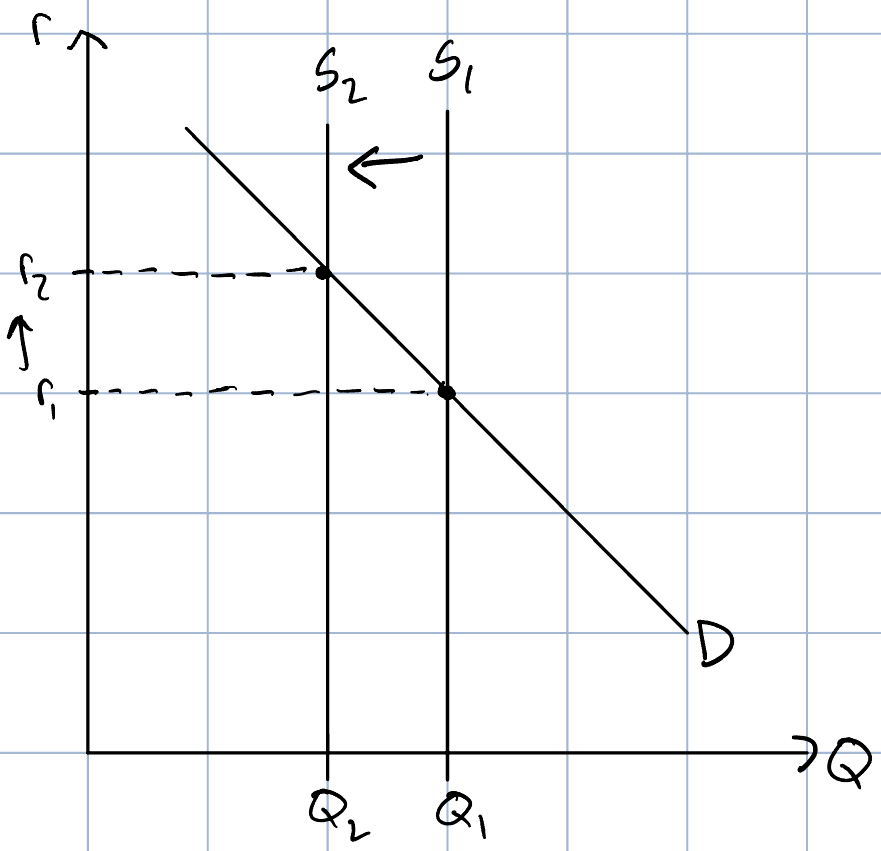
\includegraphics[width = 0.4\textwidth]{qq2}
	\end{center}

\item (b) -- When the Fed sets an interest rate target, it commits to holding the interest rate fixed rather than the money supply fixed. In order to hold the interest rate fixed, it has to adjust the supply of money to offset any changes in the demand for money.

\item (b) -- Increasing government purchases directly increases aggregate demand. Decreasing taxes makes households feel richer, so it increases consumption.

\item (d) -- The multiplier is \[\frac{1}{1 - \frac{2}{3}} = 3,\] so the increase in aggregate demand is $\$1,200 \cdot 3 = \$3,600.$

\item (c) -- The increase in government spending would increase household income and consumption. The increase in consumption would increase the demand for money. If the Fed held the money supply constant, the interest rate would increase. That would decrease investment, so some of the increase in aggregate demand would be offset by the crowding out effect.

\item (d) — If the Fed decreased the interest rate, it would increase investment. If Congress decreased taxes, it would increase investment. Both would shift aggregate demand to the right and offset the leftward shift due to pessimism. 

\item (d) — Firms take a long time to make and implement their investment plans, so there’s a lag between interest rates changing and investment responding.

\item (a) — When more people become unemployed, they automatically become eligible for unemployment insurance, so government spending increases with no need for a change in monetary or fiscal policy.

\end{enumerate}

\section*{Questions for Review}

\begin{enumerate}

\item The theory of liquidity preference is a model for explaining short-run interest rates using the money market. First, it says that the supply of money is fixed by the Fed. Second, it says the demand for money decreases as the interest rate increases because the interest rate is the opportunity cost of holding money. 

	\begin{center}
	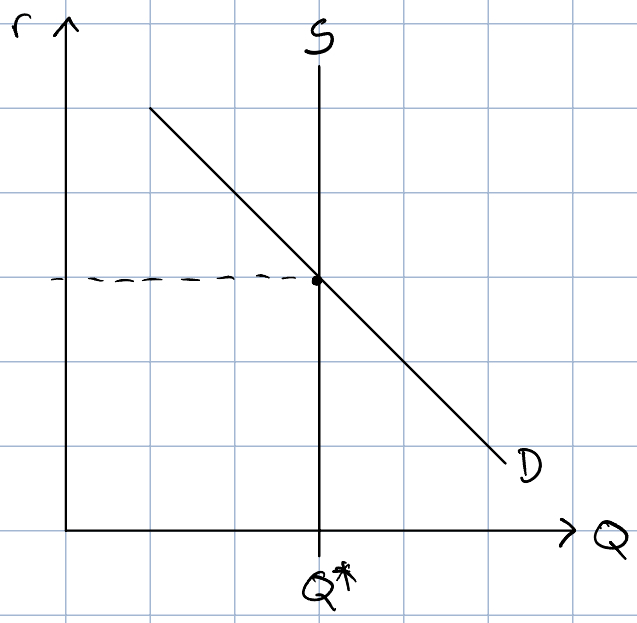
\includegraphics[width = 0.4\textwidth]{qfr1a}
	\end{center}

It helps explain the downward slope of the aggregate-demand curve using the interest rate effect. It says that if the price level increases, then people's demand for money will increase because they will need more money to keep up with their increased cost of living. If demand increases, that drives up the interest rate. A higher interest rate increases the cost of borrowing which in turn decreases investment. Lower investment means lower demand. 

	\begin{center}
	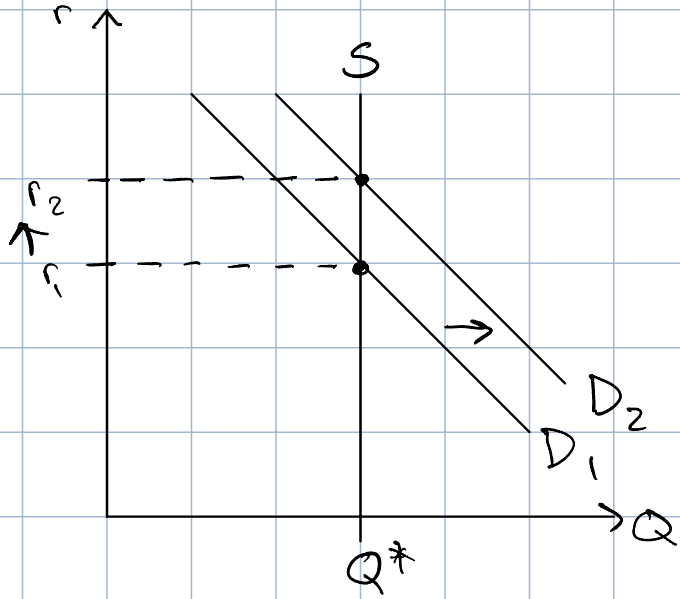
\includegraphics[width = 0.4\textwidth]{qfr1b}
	\end{center}

\item If the money supply decreases, the interest rate increases.

	\begin{center}
	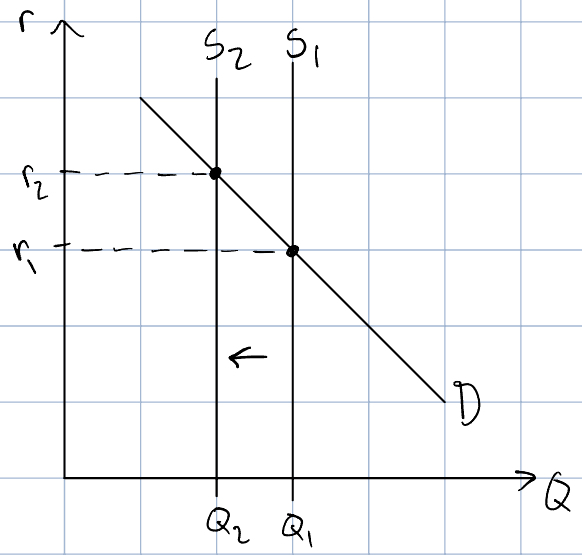
\includegraphics[width = 0.4\textwidth]{qfr2a}
	\end{center}
	
	If the interest rate increases, that increases the cost of borrowing which in turn decreases investment. If investment decreases, aggregate demand shifts left.
	
	\begin{center}
	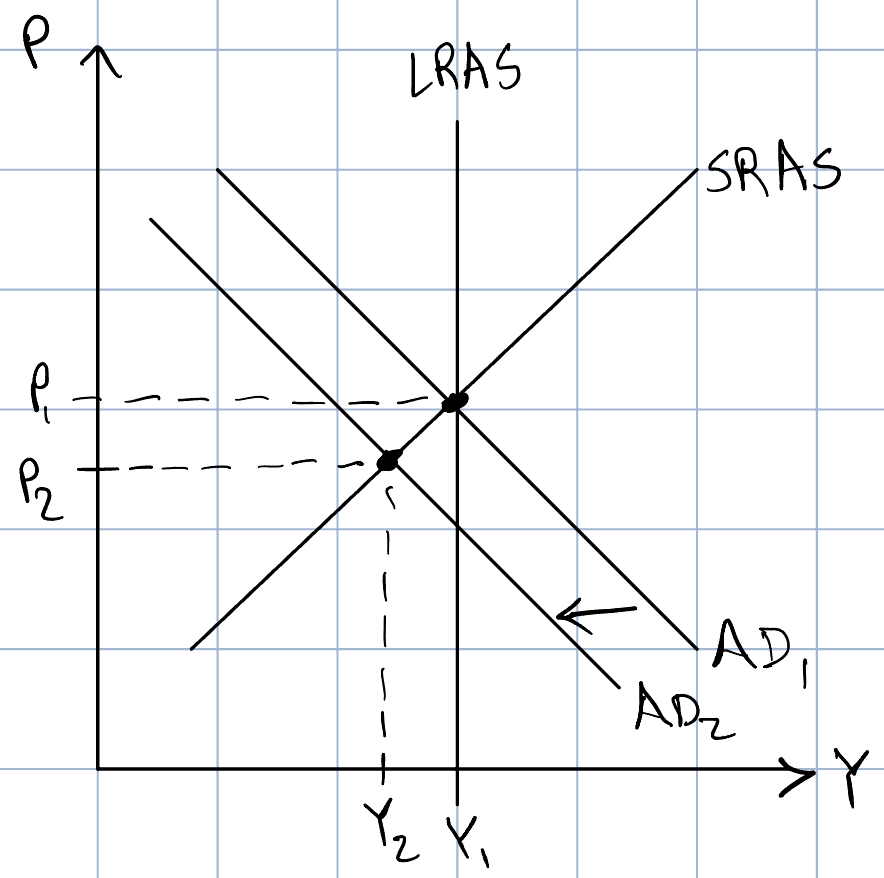
\includegraphics[width = 0.4\textwidth]{qfr2b}
	\end{center}

\item If the government spends \$3 billion on police cars, police car producers' incomes increase. Higher incomes cause those producers to consume more. That consumption in turn increases other producers' incomes at which point those producers will consume more. Therefore, the government spending sparks additional consumption which creates a multiplier effect. Additionally, the increase in demand could encourage firms to invest more, so there could also be an investment accelerator. As a result, aggregate demand could increase by more than \$3 billion.

When government spending boosts household income and consumption, households need to hold more money for their additional purchases. That increases the demand for money which increases the interest rate (if the Fed doesn't increase the money supply in response). A higher interest rate decreases investment, so government spending could crowd out private investment and partially offset the increase in aggregate demand. As a result, aggregate demand could increase by less than \$3 billion. 

\item A wave of pessimism will decrease consumption and investment. If policymakers do nothing, aggregate demand will shift left.

If the Fed wants to stabilize the economy, it will need to increase the money supply so that the interest rate falls and investment increases. That will shift the aggregate demand curve back to the right.

If the Fed does nothing, Congress could increase spending or decrease taxes. Increasing spending would increase government purchases. It would also increase consumption due to the multiplier effect and act as an investment accelerator if firms respond to increased demand by increasing investment. Decreasing taxes would increase household consumption because households would feel richer. Both changes would shift aggregate demand back to the right.  

\item Unemployment insurance is an automatic stabilizer. When people get laid off, the government pays them a portion of their old salary while they look for another job. Those payments are called unemployment insurance. Since unemployment increases during recessions, unemployment insurance payments increase during recessions. That means government spending automatically increases when a recession hits.

\end{enumerate}

\section*{Problems \& Applications}

\begin{enumerate}

\item

	\begin{enumerate}
	
	\item If the Fed buys bonds, the supply of money shifts right. As a result, the quantity of money supplied and demanded increases, and the interest rate decreases.

		\begin{center}
		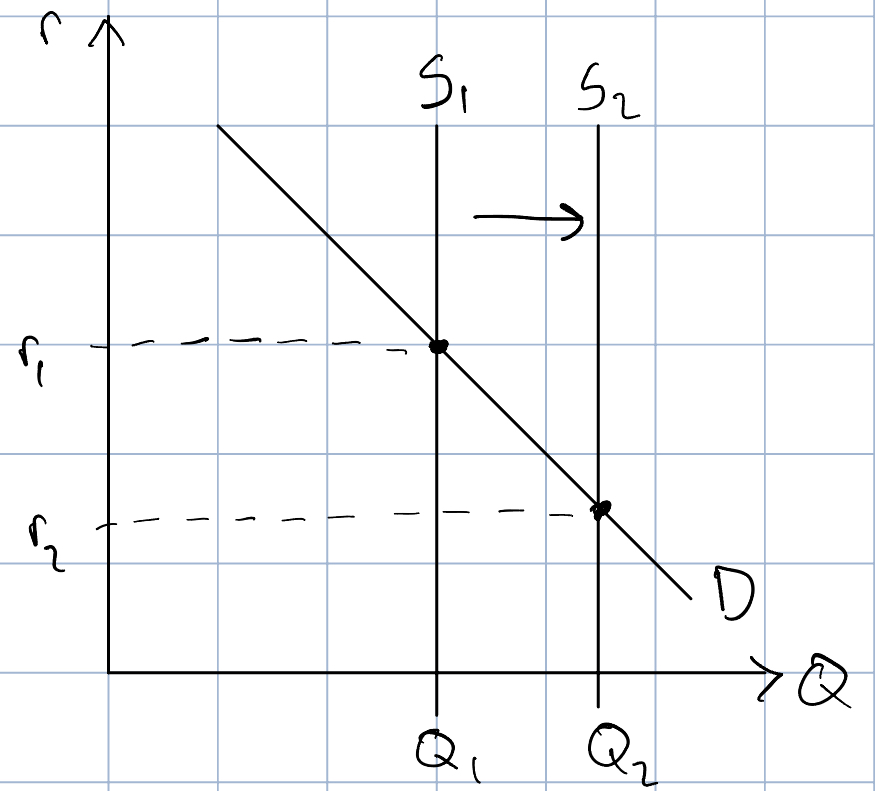
\includegraphics[width = 0.4\textwidth]{paa1a}
		\end{center}

	\item If people want to hold less cash, the demand for money shifts left. The quantity of money supplied and demanded remain constant, but the interest rate decreases.

		\begin{center}
		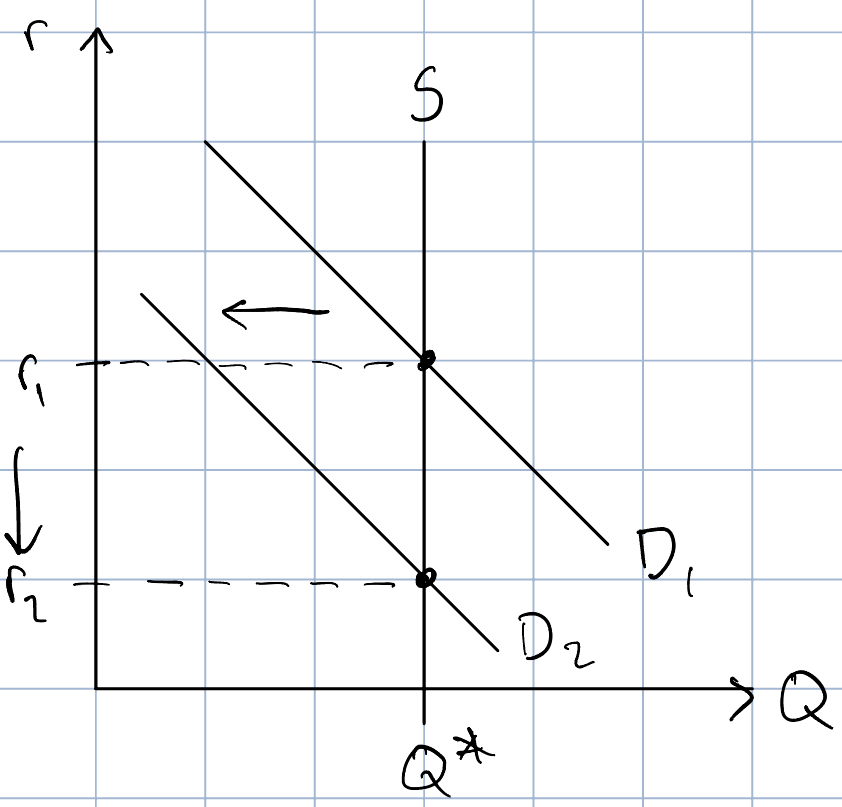
\includegraphics[width = 0.4\textwidth]{paa1b}
		\end{center}

	\item If the Fed reduces the interest rate it pays on reserves, the supply of money shifts right. As a result, the quantity of money supplied and demanded increases, and the interest rate decreases.
	
		\begin{center}
		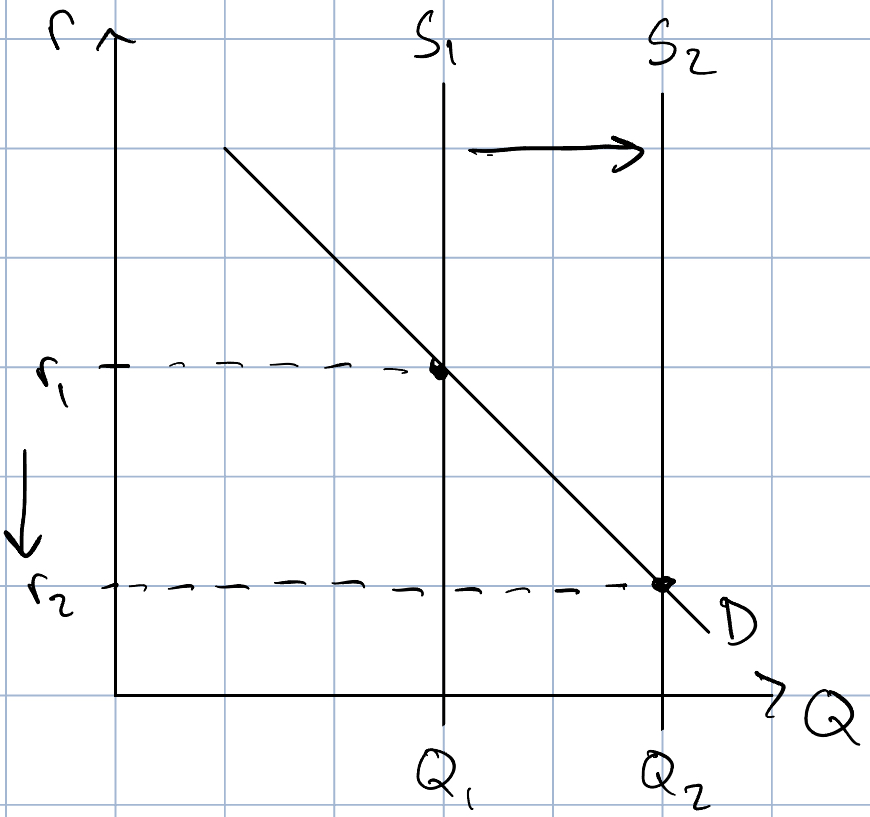
\includegraphics[width = 0.4\textwidth]{paa1c}
		\end{center}
		
	\item If households decide to hold more money, the demand for money shifts right. The quantity of money supplied and demanded remain constant, but the interest rate increases.
	
		\begin{center}
		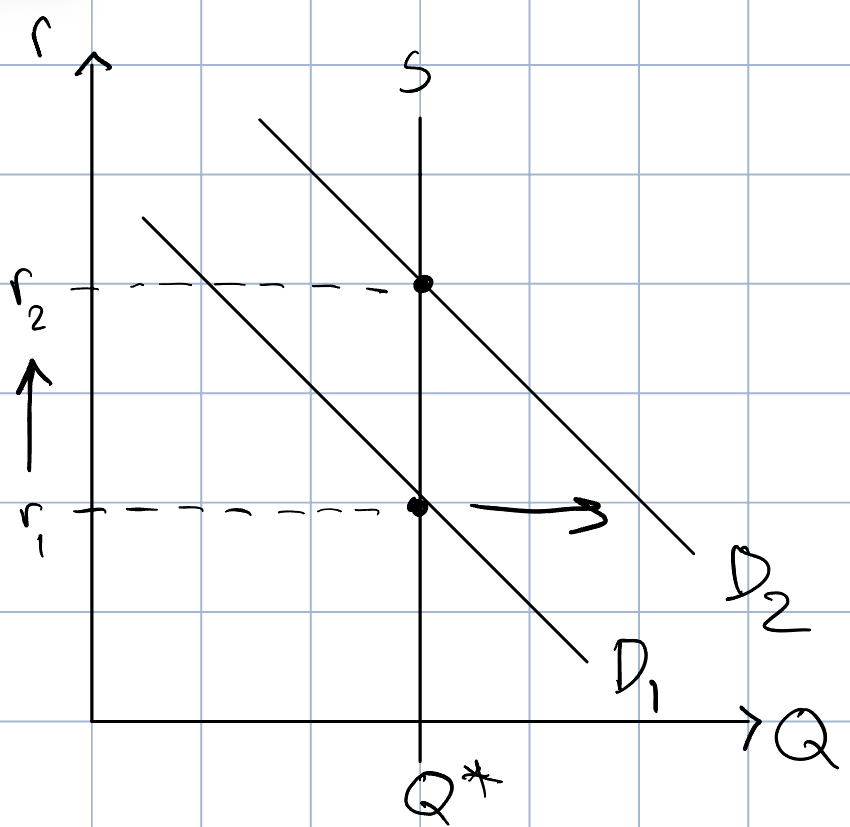
\includegraphics[width = 0.4\textwidth]{paa1d}
		\end{center}
		
	\item If aggregate demand shifts right, the price level increases. As a result, people need to hold more money, so the demand for money shifts right. The quantity of money supplied and demanded remain constant, but the interest rate increases.
	
		\begin{center}
		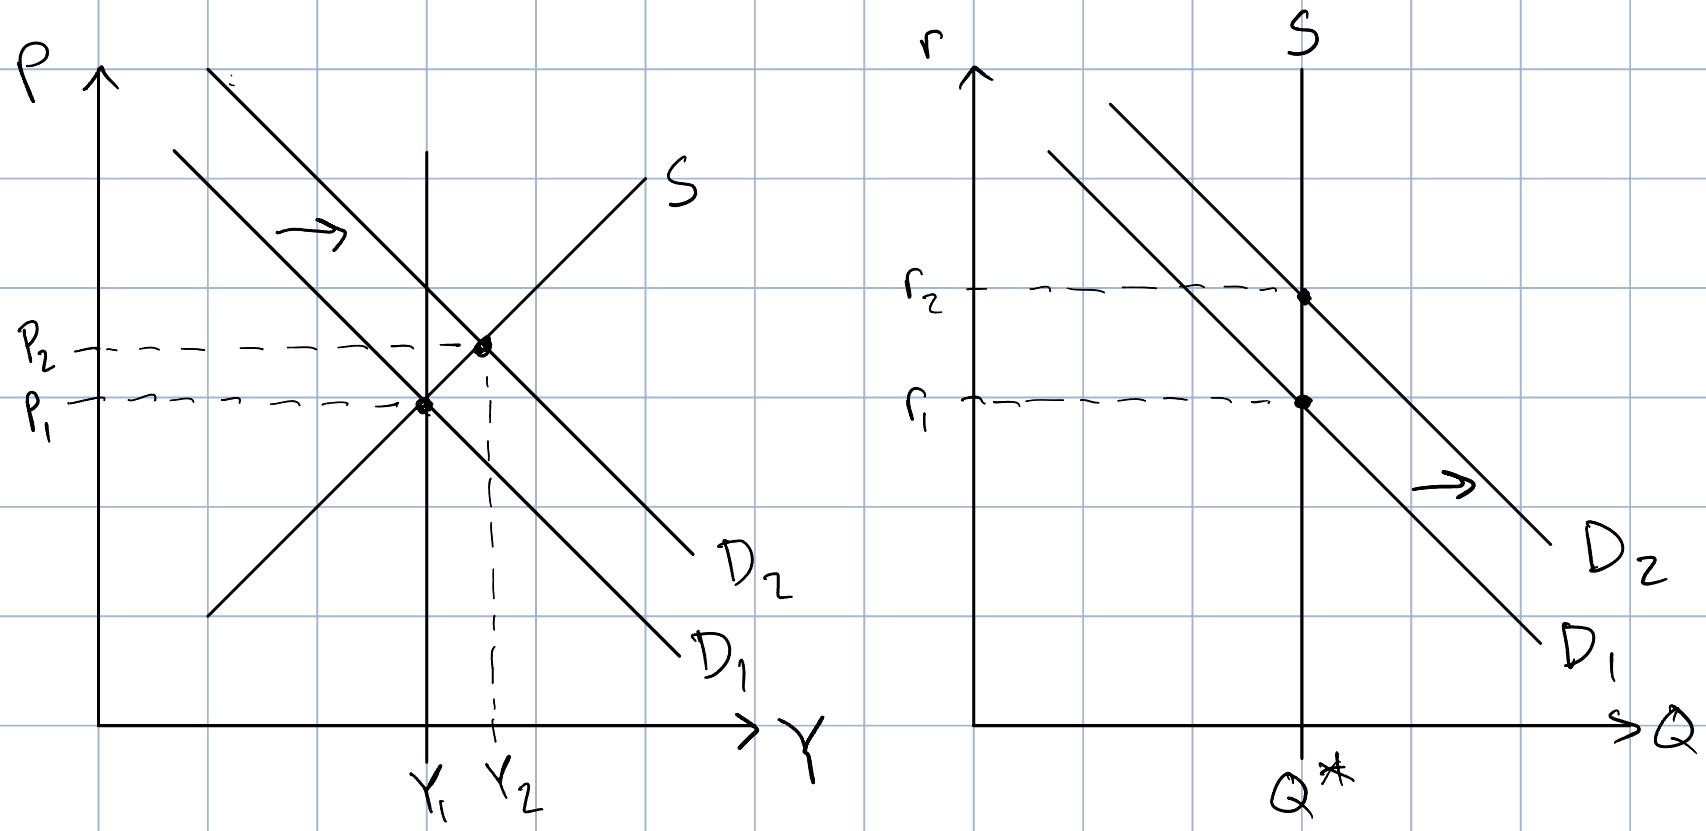
\includegraphics[width = 0.8\textwidth]{paa1e}
		\end{center}
	
	\end{enumerate}

\item

	\begin{enumerate}
	
	\item The supply of money shifts right, so the interest rate decreases.
	
		\begin{center}
		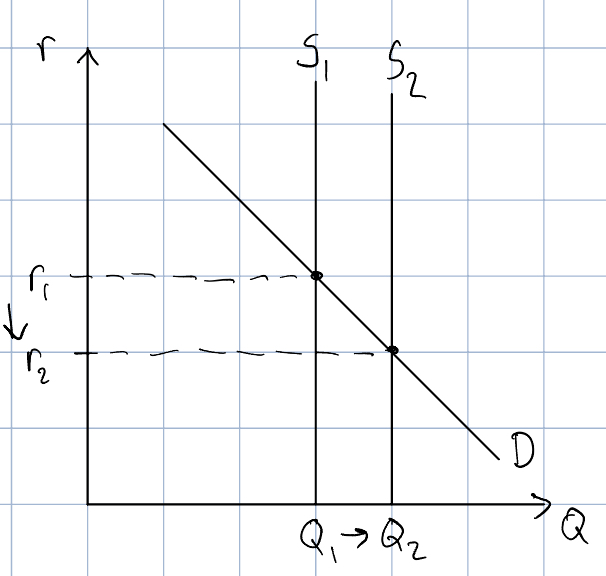
\includegraphics[width = 0.5\textwidth]{paa2a}
		\end{center}
		
	\item A lower interest rate stimulates investment, so aggregate demand shifts right. That increases the price level and output.
		
		\begin{center}
		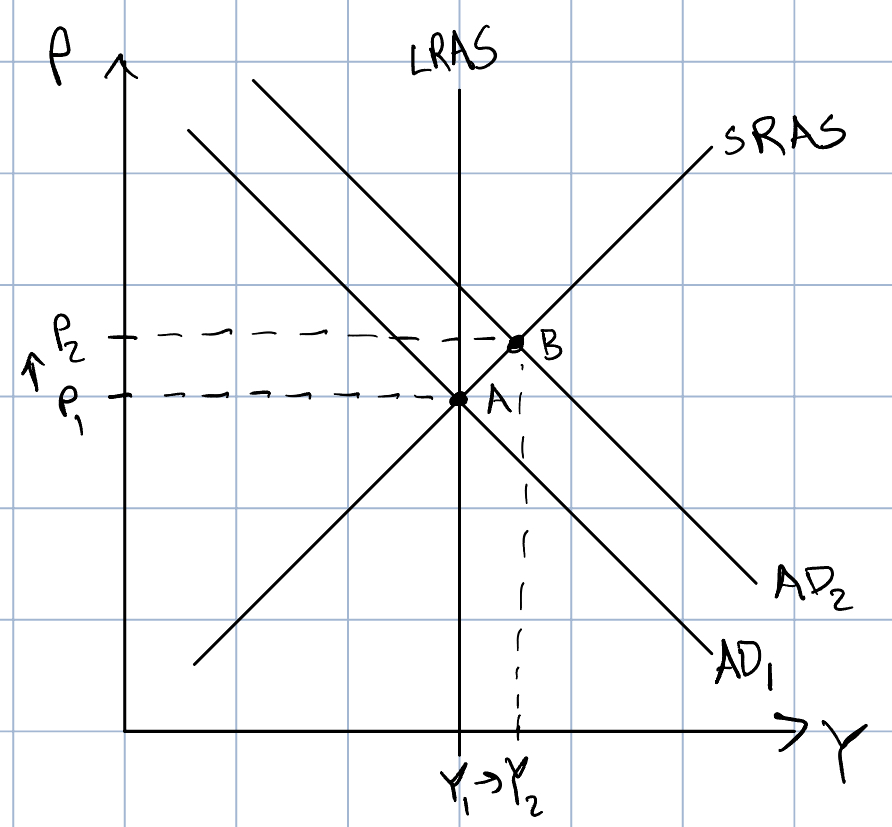
\includegraphics[width = 0.5\textwidth]{paa2b}
		\end{center}
		
	\item The short-run aggregate supply curve will shift left to return the economy to long-run equilibrium, so the price level will increase.
	
		\begin{center}
		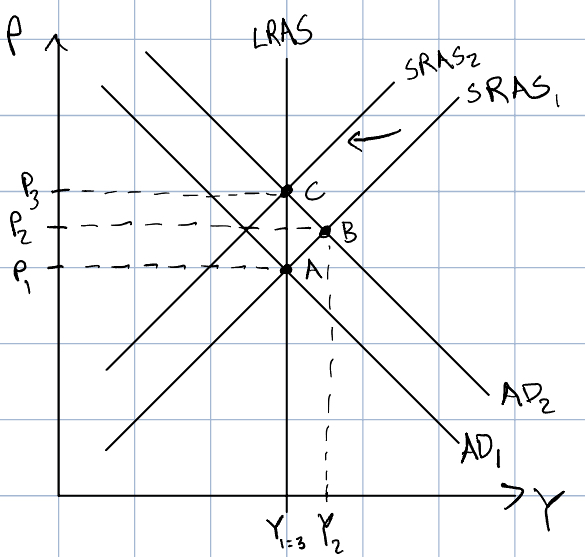
\includegraphics[width = 0.5\textwidth]{paa2c}
		\end{center}
		
	\item When the price level increases, people need to hold more money to pay for their expenses. That shifts the demand for money right. When the demand for money shifts right, the interest rate increases.
	
		\begin{center}
		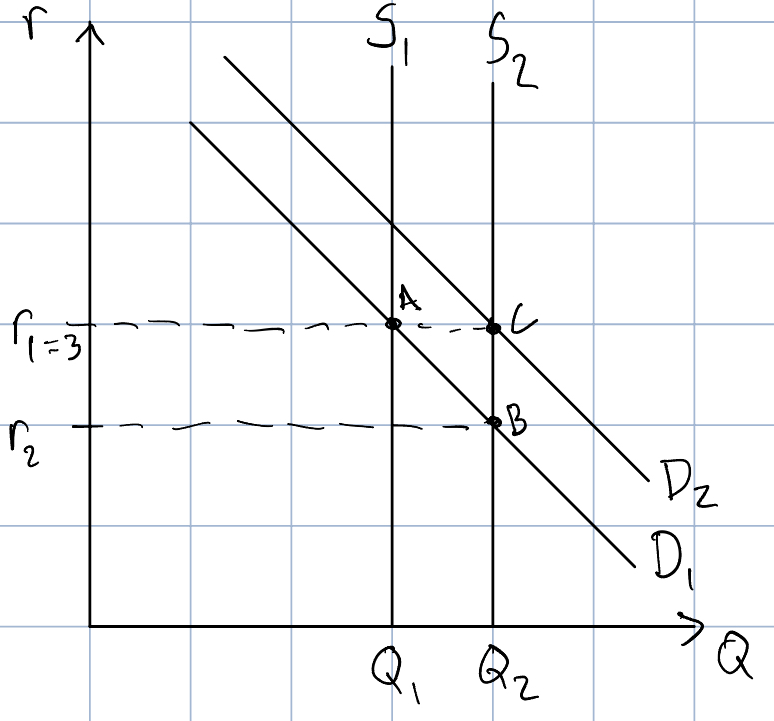
\includegraphics[width = 0.4\textwidth]{paa2d}
		\end{center}
		
	\item This is consistent with the proposition that money has real effects in the short run but is neutral in the long run. In the short run, the interest rate, investment, and aggregate output increased. In the long run, all three return to their original level, and the only thing that changes is the price level.
	
	\end{enumerate}

\item

	\begin{enumerate}
	
	\item If the demand for money shifts right, the interest rate increases. As a result, investment decreases, and aggregate demand shifts left.
	
		\begin{center}
		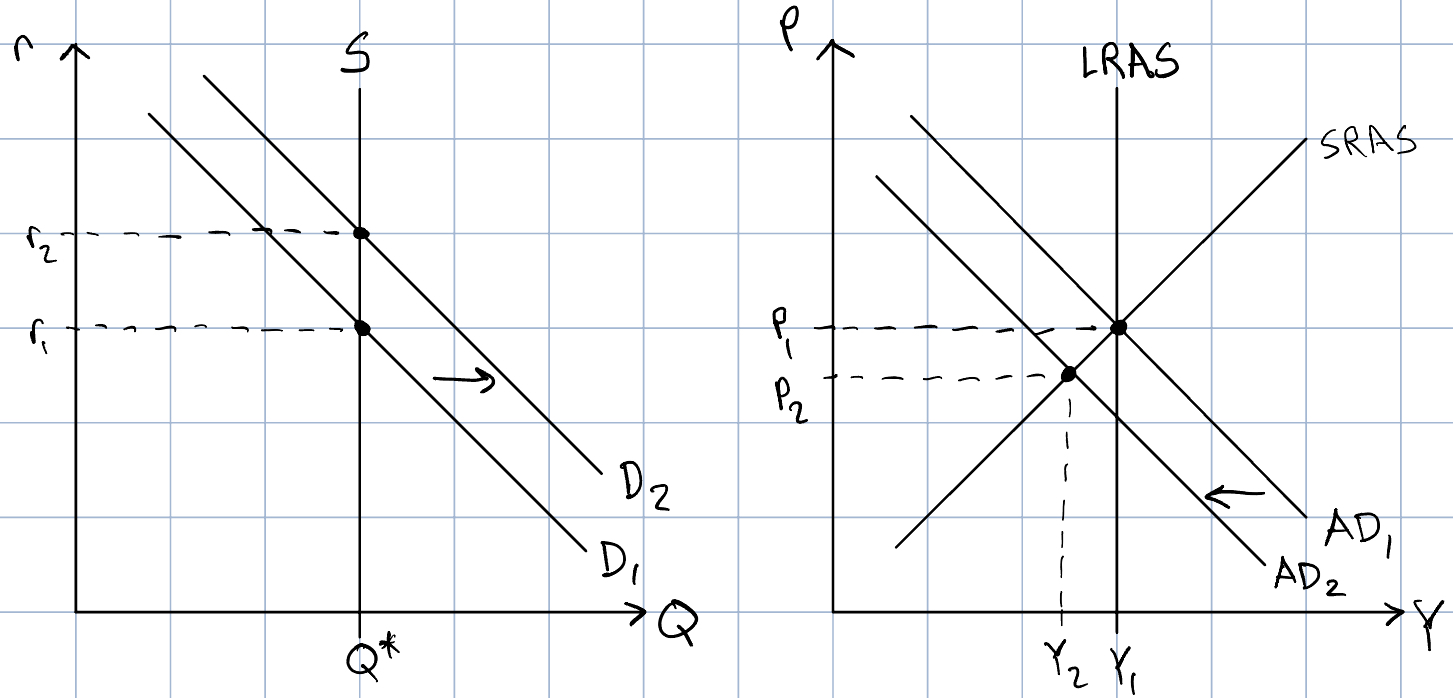
\includegraphics[width = 0.9\textwidth]{paa3a}
		\end{center}
	
	\item The Fed should increase the money supply.
	
		\begin{center}
		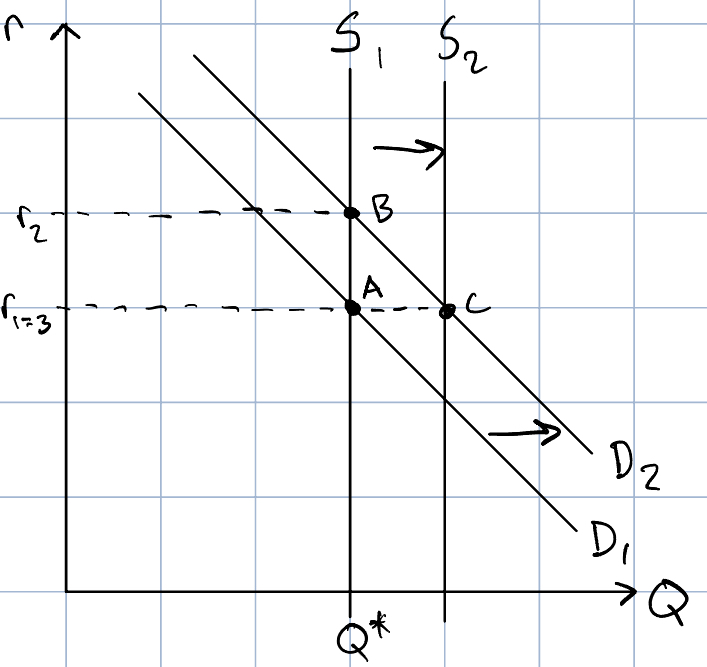
\includegraphics[width = 0.4\textwidth]{paa3b}
		\end{center}
	
	\item It should buy bonds.
	
	\end{enumerate}

\item The permanent policy will stimulate greater spending because consumers will perceive it as a larger increase in their wealth. Because the permanent policy stimulates greater spending, it causes a larger rightward shift in aggregate demand.

\item

	\begin{enumerate}
	
	\item You could draw this as a leftward shift in AD or SRAS. Here, I've drawn it as a leftward shift in AD.
	
		\begin{center}
		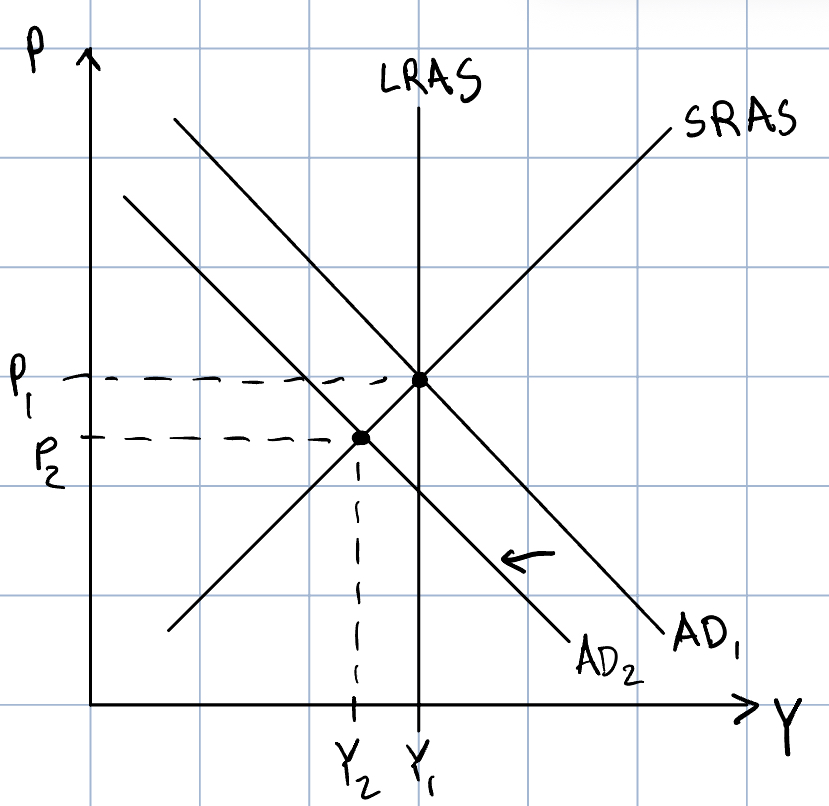
\includegraphics[width = 0.9\textwidth]{paa5a}
		\end{center}
	
	\item The Fed could buy bonds to increase the supply of money.
	
	\item \phantom{x}
	
		\begin{center}
		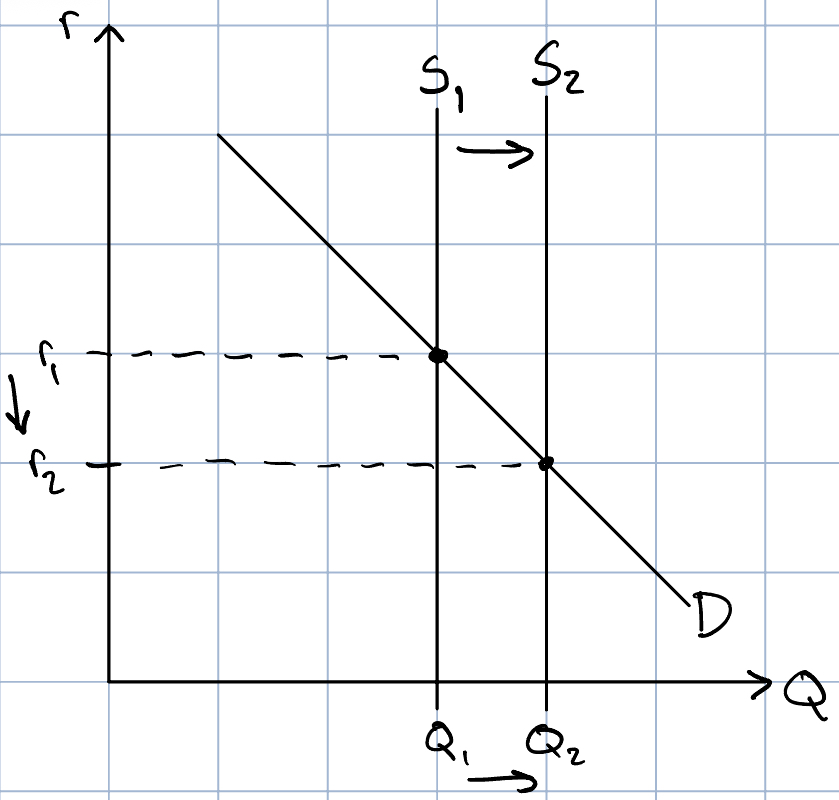
\includegraphics[width =0.4\textwidth]{paa5b}
		\end{center}
	
	\item When the Fed increases the supply of money, the interest rate falls. That stimulates investment which in turn increases aggregate demand.
	
		\begin{center}
		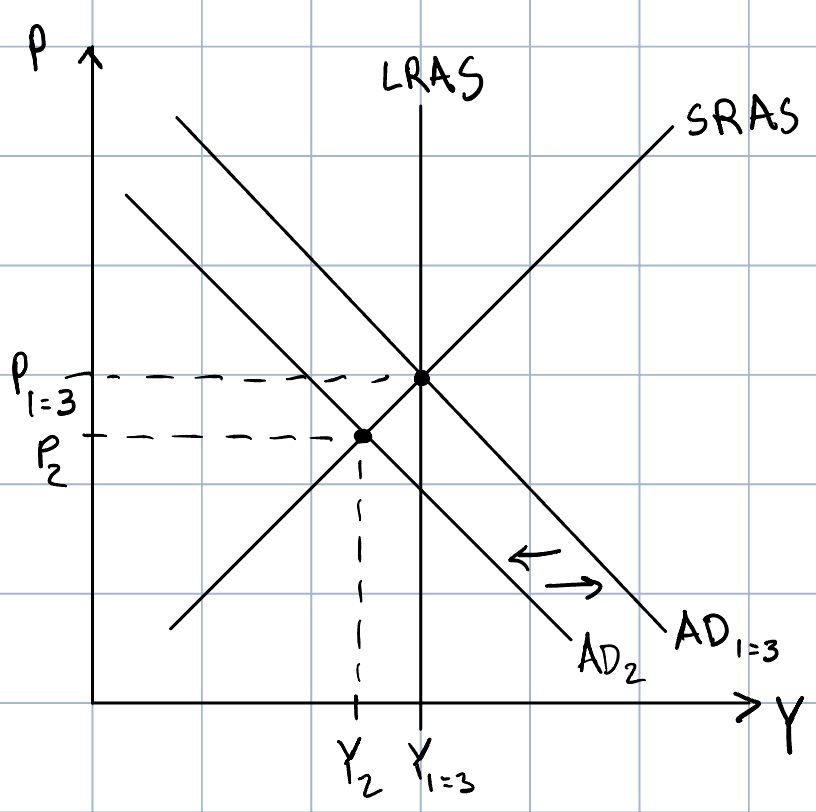
\includegraphics[width = 0.4\textwidth]{paa5c} 
		\end{center}
	
	\end{enumerate}

\item

	\begin{enumerate}
	
	\item If people could earn interest on their money, that would increase their incentive to hold money. As a result, money demand would increase.
	
	\item The interest rate would have increased. That would discourage investment, so aggregate demand would shift left. That would decrease aggregate output.
	
		\begin{center}
		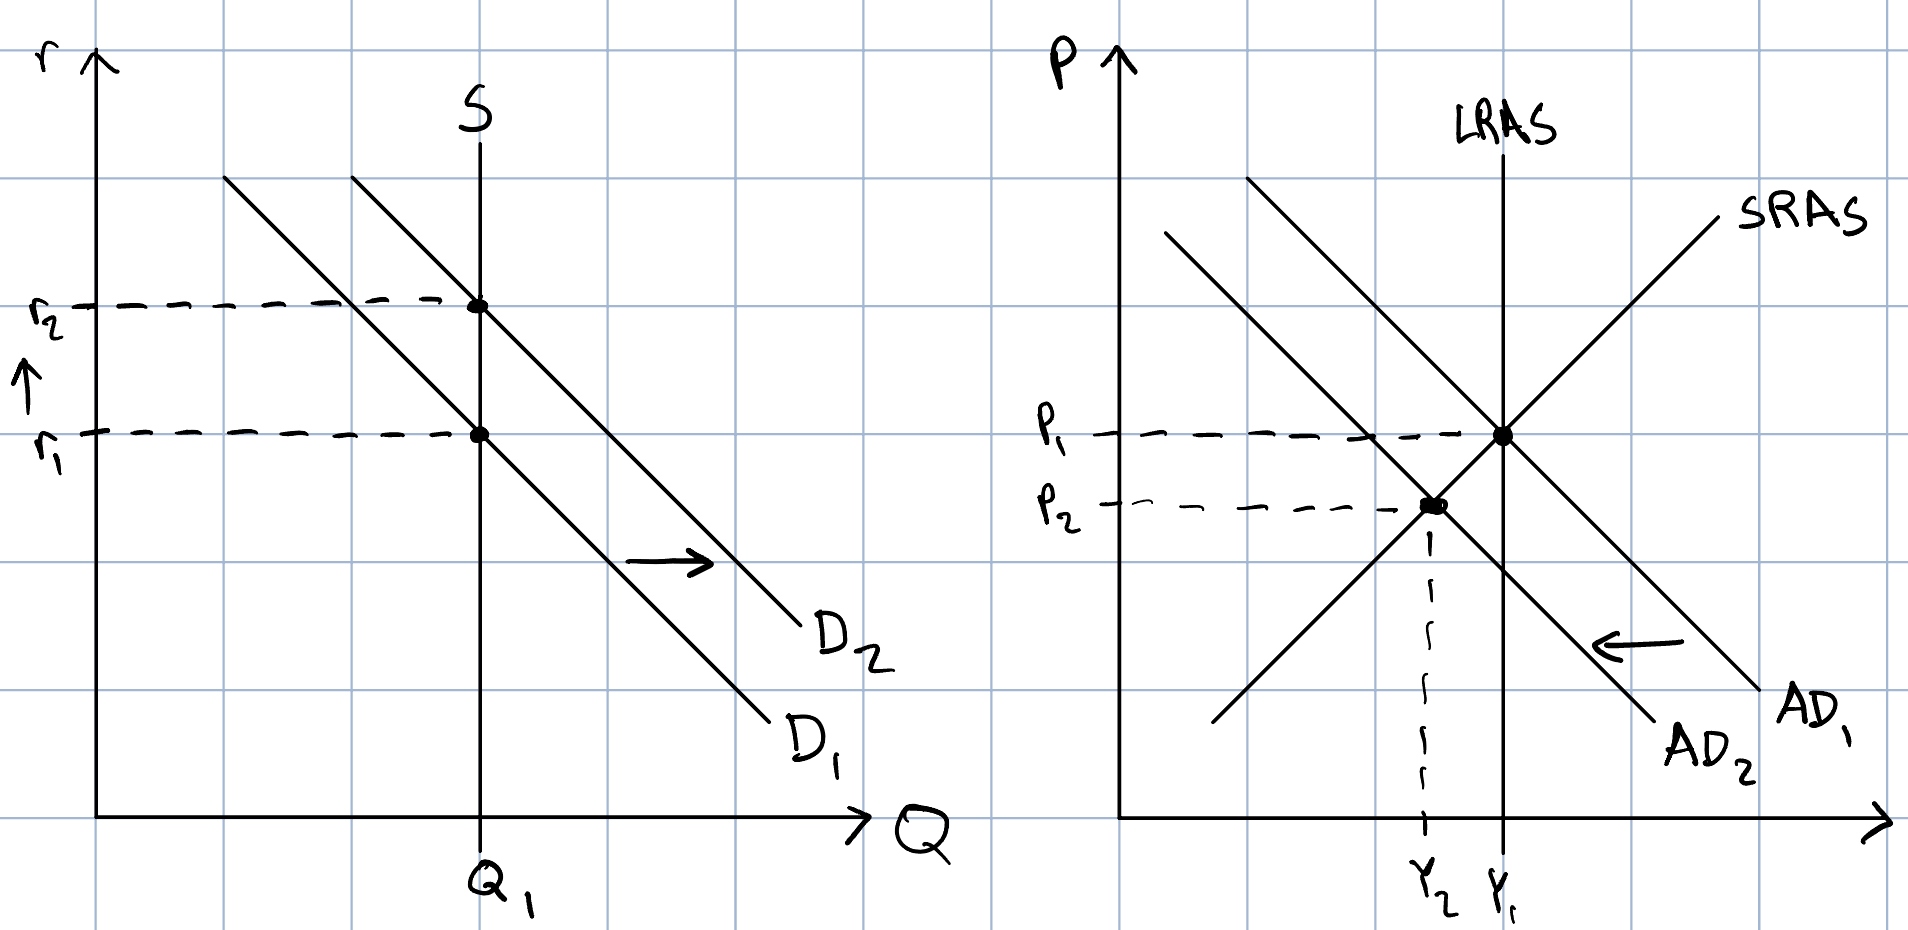
\includegraphics[width = 0.9\textwidth]{paa6b}
		\end{center} 
	
	\item The Fed would have had to increase the supply of money. If they had, aggregate demand and aggregate output would have remained constant.
	
		\begin{center}
		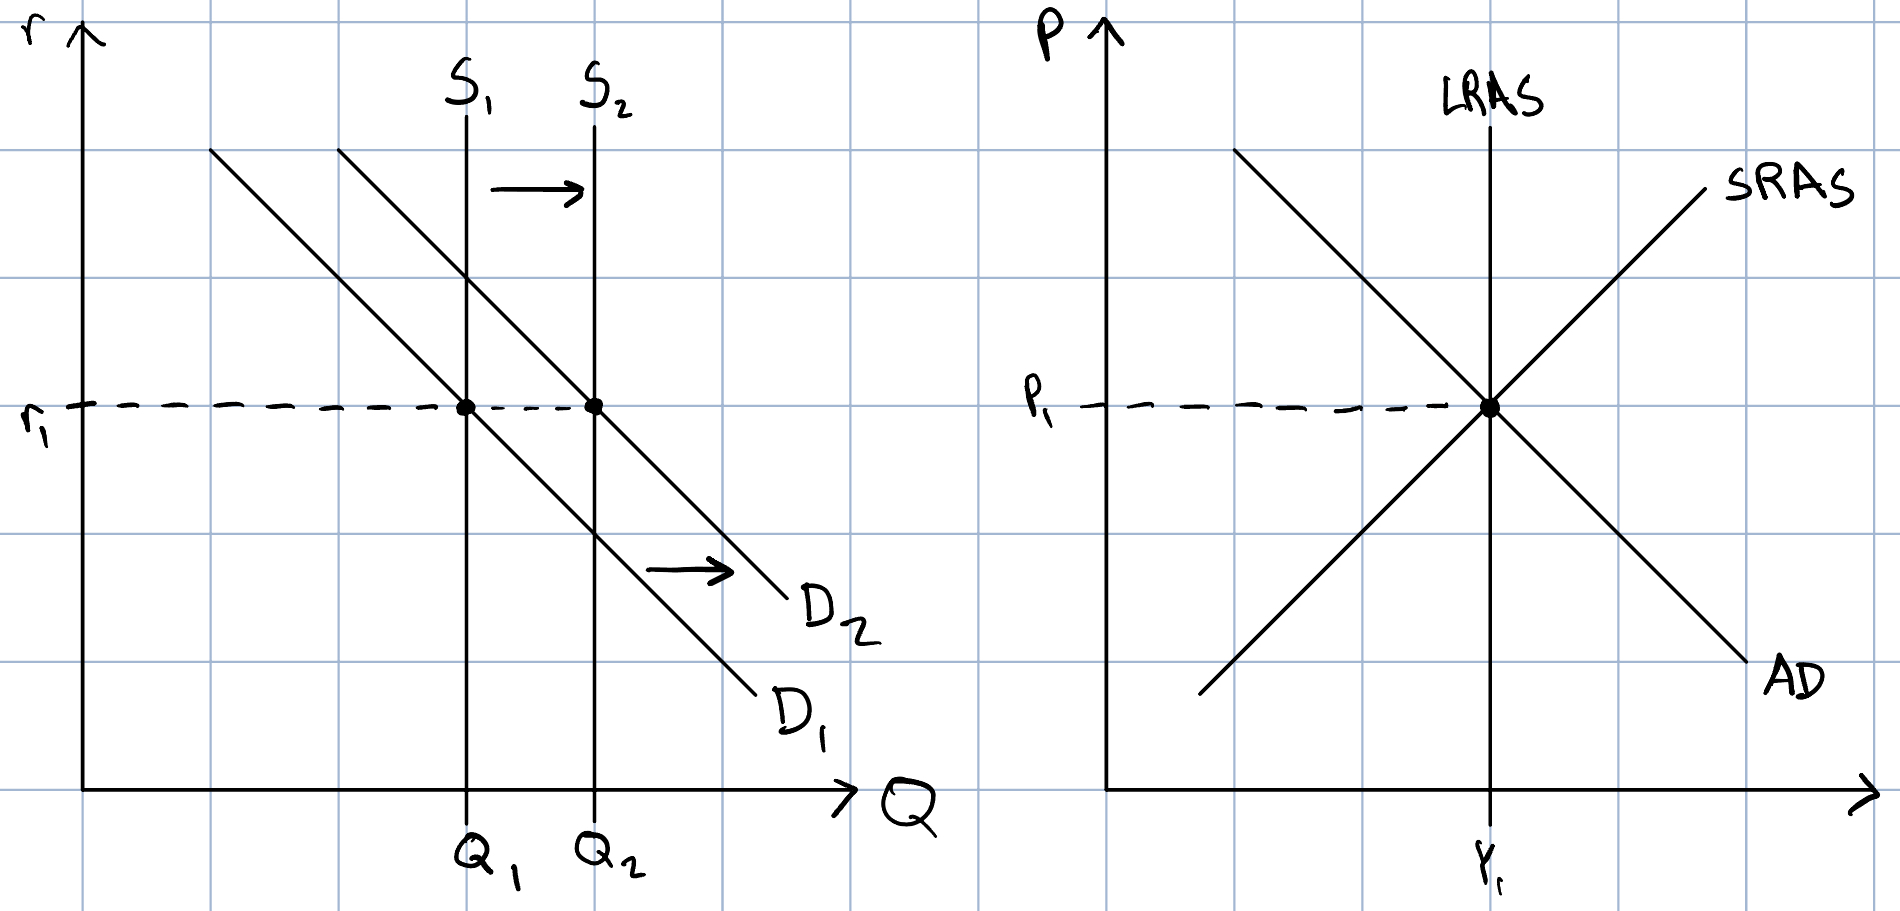
\includegraphics[width = 0.9\textwidth]{paa6c}
		\end{center}
	
	\end{enumerate}

\item 

	\begin{enumerate}
	
	\item The multiplier is $30 / 10 = 3$. Therefore, the MPC is
	
		\begin{gather*}
		3 = \frac{1}{1 - \text{MPC}} \\
		3 - 3\text{MPC} = 1 \\
		2 = 3\text{MPC} \\
		\frac{2}{3} = \text{MPC}
		\end{gather*}
	
	\item Their new estimate of the MPC would be larger. If some investment is crowded out, that offsets some of the multiplier effect. That means the multiplier is actually greater than three in which case people must increase their consumption more than the MPC of $2/3$ indicates.
	
	\end{enumerate}

\item If the MPC is $4/5$, then the multiplier effect is
	\[ \frac{1}{1 - \frac{4}{5}} = 5. \]
	That means for every dollar that the government spends, it creates \$5 of additional consumption. Therefore, the government needs to increase its spending by \[\frac{\$400 \text{ billion}}{5} = \$80 \text{ billion}\] in order to boost aggregate demand by \$400 billion total.

\item The effect on aggregate demand would be larger if the Fed committed to maintaining a fixed interest rate. Government spending generates additional income for households. That increases their consumption which in turn increases their demand for money. If the Fed holds the money supply constant, the increase in demand for money will increase the interest rate and decrease investment. That crowding out will partially offset the increase in aggregate demand from the increase in government spending. If the Fed holds the interest rate fixed, there won't be any crowding out.

\item 

	\begin{enumerate}
	
	\item It is more likely to lead to a short-run increase in investment when the investment accelerator is large. If the government increases its spending, aggregate demand increases. When the investment accelerator is large, firms increase their investment more in response to an increase in demand.
	
	\item It is more likely to lead to a short-run increase in investment when the interest sensitivity of investment is small. If the Fed doesn't change the money supply, the increase in government spending will increase interest rates because households will have higher incomes, consume more, and therefore demand more money. An increase in interest rates will crowd out investment more if interest sensitivity is high.
	
	\end{enumerate}

\item

	\begin{enumerate}
	
	\item The first equation shows that GDP has three components -- consumption, investment, and government spending -- which means the economy is closed. The second equation shows how consumption depends on after-tax income. The third equation shows how investment depends on interest rates. The fourth and fifth equations show that government spending and taxes are fixed.
	
	\item The MPC in this economy is 0.75 because when income ($Y$) increases by 1, consumption ($C$) increases by 0.75.
	
	\item If $r = 4$, then $I = 500 - 50(4) = 300$. Therefore, GDP is
		\begin{align*}
		Y &= C + I + G \\
		Y &= 100 + 0.75(Y - 100) + 300 + 125 \\
		Y &= 450 + 0.75Y \\
		0.25Y &= 450 \\
		Y &= 1,800.
		\end{align*}
		That's \$200 less than the full-employment level.
		
	\item Since the MPC is 0.75, the multiplier is 
		\[\frac{1}{1 - 0.75} = 4.\]
		Therefore, the government needs to increase spending by $\$200/4 = \$50$ to restore full employment.
		
	\item Decreasing the interest rate to 3\% would restore full employment.
		\begin{align*}
		Y &= C + I + G \\
		Y &= 100 + 0.75(Y - 100) + 500 - 50r + 125 \\
		2,000 &= 100 + 0.75(2,000 - 100) + 500 - 50r + 125 \\
		2,000 &= 2,150 - 50r \\
		50r &= 150 \\
		r &= 3
		\end{align*}
	
	\end{enumerate}
	
\end{enumerate}

\end{document}